Se separó el programa por capas, siendo la \textbf{App} la principal y subdividiendo la capa de \textbf{Drivers} en las capas de \textbf{HAL} y \textbf{MCAL}. Dicha separación puede verse con detalle en la Figura~(\ref{fig:drivers}), donde se muestra como la \textbf{App} entra en contacto únicamente con los drivers de la placa de desarrollo \textbf{FRDM}, de la \textbf{Placa Verde} y con el \textbf{Lector} de la tarjeta.
 
\begin{figure}[H]
\centering
	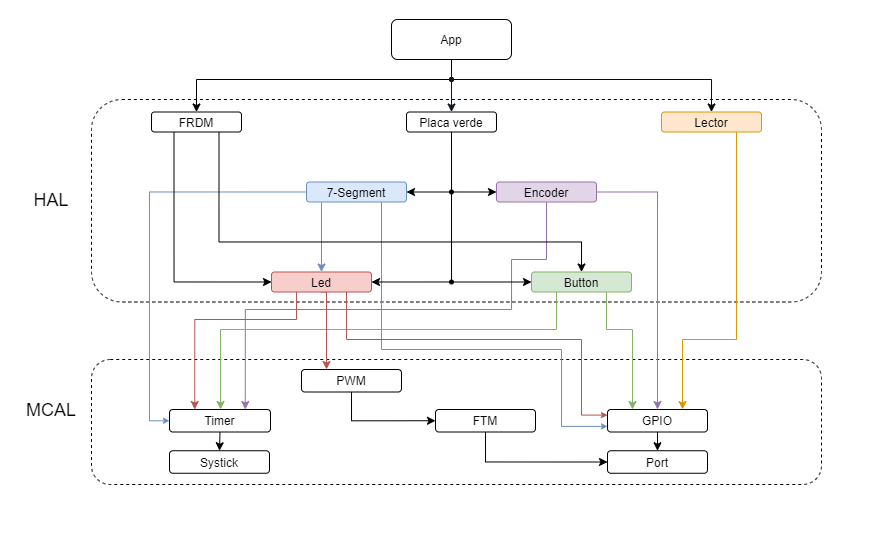
\includegraphics[width=0.9\textwidth]{ImagenesEjercicio3/esquema_drivers.png}
	\caption{Arquitectura del firmware, jerarquía y relación entre los módulos.}
	\label{fig:drivers}
\end{figure}

El driver \textbf{FRDM} emplea los drivers de \textbf{Led} y \textbf{Button}, mientras que la \textbf{Placa Verde}, ademas de los dos recién mencionados, se vale del uso de los drivers de \textbf{Encoder} y del \textbf{7 Segment}. Todos los mencionados junto con el \textbf{Lector} conforman la Hardware Abstraction Layer.

Por otro lado, la Microcontroller Abstraction Layer se encuentra conformada por los drivers de \textbf{Timer}, \textbf{PWM}, \textbf{Gpio}, \textbf{FTM}, \textbf{Systick} y \textbf{Port}, siendo estos últimos 3 los únicos que no tienen contacto con drivers de la HAL. 

En la Figura~(\ref{fig:drivers}) se puede apreciar la interconexión entre drivers de las distintas capas, diferenciando por colores las distintas dependencias entre la HAL y la MCAL para un mejor entendimiento.